\documentclass[12pt,letterpaper]{article}
\usepackage[latin1]{inputenc}
\usepackage[spanish]{babel}
\usepackage{amsmath}
\usepackage{amsfonts}
\usepackage{amssymb}
\usepackage{graphicx}
\usepackage[hidelinks]{hyperref}
\usepackage{color}
\graphicspath{{Imagenes/}}
\usepackage[left=2cm,right=2cm,top=2cm,bottom=2cm]{geometry}
\author{M�rquez M�rquez Amairani Ivette}
\begin{document}
\begin{center}
\textbf{\huge {Universidad Politecnica de la Zona \\[0.5cm] Metropolitana de Guadalajara}}
\end{center}

\begin{center}

\includegraphics[width=0.65\textwidth]{Imagenes/UPCDLZMDG5783-logo.png}\\[2cm] 
\end{center}
\vspace{0.1cm}
{\large\textbf{Evidencia:} 2.4 Giro de un motor corriente directa\\[0.2cm]\textbf{Alumna:} M�rquez M�rquez Amairani Ivette\\[0.2cm]\textbf{Profesor:} M�ran Garabito Carlos Enrique\\[0.2cm]\textbf{Carrera:} Ing.Mecatronica\\[0.2cm]\textbf{Grupo:} 4�B\\[0.2cm]\textbf{Fecha de entrega:} 15 de Octubre del 2019\\[0.2cm]\\

\vspace{10cm}
\textbf{2.4 Giro de un motor de corriente directa}\\[0.3cm]
El principio de funcionamiento de los motores de corriente directa se basa en la repulsi�n que ejercen los polos magn�ticos de un im�n permanente cuando, de acuerdo con la Ley de Lorentz, interact�an con los polos magn�ticos de un electroim�n que se encuentra montado en un eje. Este electroim�n se denomina rotor y su eje le permite girar libremente entre los polos magn�ticos norte y sur del im�n permanente situado dentro de la carcasa o cuerpo del motor.\\

En la figura 1 se muestra, de forma esquem�tica y simplificada, un motor com�n de corriente directa (C.D.) con un rotor formado por una simple bobina de una sola espira de color rojo y azul, para diferenciar cada mitad. Si seguimos el recorrido de la corriente el�ctrica (I) asumiendo que fluye en el sentido convencional (del polo positivo, al polo negativo  de la bater�a, seg�n indican las flechas negras), cuando en la mitad izquierda de la espira de color rojo se forma el polo norte (N) coincidiendo con la misma polaridad del campo magn�tico del im�n permanente fijo al cuerpo del motor, se produce una fuerza de rechazo entre ambos polos iguales.
 
 \begin{figure}[h]
\centering
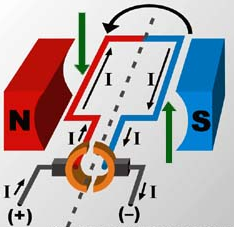
\includegraphics[width=0.50\textwidth]{Imagenes/2.PNG}
\caption{Motor com�n de corriente directa}
\label{fig:Motor}
 \end{figure}

 {\large\textbf{Bibliograf�a}\\
 \emph{Garc�a.A(09 del 2015). As� funciona un motor en corriente directa.}
 Obtenido de:
 \textcolor{blue}{http://www.asifunciona.com}\\[0.3cm]

\end{document}